%  Typ dokumentu - článek, prezentace aj.
\documentclass[english]{article}

%  Nastaví vstupní a výstupní kódování znaků (encoding) a lokalizace
\usepackage[T1]{fontenc}
\usepackage[utf8]{inputenc}
\usepackage[english,czech]{babel}
\usepackage{icomma}
\usepackage{lmodern}

%  Formát papíru a odsazení od jeho okrajů
\usepackage[letterpaper]{geometry}
\geometry{verbose,tmargin=1.5cm,bmargin=2cm,lmargin=2cm,rmargin=2cm}

%  Umožňuje pracovat s grafikou
\usepackage{graphicx}

%  Automaticky odsadí i první paragraf v každé sekci
\usepackage{indentfirst}

%  Umožňuje rozdělovat obsah na více sloupců
\usepackage{multicol}

%  Umožňuje používat hypertextové odkazy, nastavuje jejich barvu a
%  vlastnosti
\usepackage{hyperref}
\hypersetup{
colorlinks=true, citecolor=blue, filecolor=blue, linkcolor=blue,
urlcolor=blue
}

%  Umožnění odstranění italiky u jednotek
\newcommand{\unit}[1]{\mathrm{#1}}

%  Formátování stránek, empty = odstraní číslování
% \pagestyle{empty}

%  Řádkování
\linespread{1.2}

%  Lepší zobrazování matematiky (rozšíření sum o \limits atd.)
\everymath{\displaystyle}

%  Velikost fontu matematických výrazů v dokumentu lze pro danou
% základního fontu dokumentu upravit pomocí:
% \DeclareMathSizes{X}{Y}{Z}{U} kde:
% X je velikost fontu v dokumentu, pro kterou se matematika upraví
% Y je standartní velikost fontu matematiky
% Z je velikost fontu zmenšených (vnořených výrazů)
% U je velikost fontu ještě více zmenšených (vnořených výrazů).
\DeclareMathSizes{10}{10.5}{9}{9}

%  Nastaví autora, název, datum, skupinu měření apod. (můj vlastní
% příkaz, umožní znovu-použití v dokumentu)
\newcommand{\Author}{David Roesel}
\newcommand{\Coauthor}{Tereza Schönfeldová}
\newcommand{\Institute}{FJFI ČVUT v Praze}
\newcommand{\Subject}{FYZIKÁLNÍ PRAKTIKUM I}
\newcommand{\Group}{7}
\newcommand{\Circle}{ZS 5}
\newcommand{\Title}{Úloha \#7 \\Rozšíření rozsahu miliampérmetru a voltmetru. Cejchování kompenzátorem.}
\newcommand{\Date}{4.10.2013}

% Začátek dokumentu - Formátování na výstup
\begin{document}

% Interní proměnné, možno zobrazovat u prezentací, používají se při
% generování pomocí \titlepage apod.
\author{\Author}
\title{\Title}
\date{\Date}

%  Lokalizace některých názvů do češtiny
\renewcommand{\figurename}{Obr.}
\renewcommand{\tablename}{Tab.}
\renewcommand{\refname}{Reference}

% --- Hlavička dokumentu -----------------------------------------------

\setlength{\parindent}{0cm}
\begin{multicols}{2}
\textbf{\Subject \\
        \Institute \\[0.1cm]
%\large  \Title \\[0.5cm]
\Title \\[0.5cm]
}
\begin{tabular}{rlrl}
\large Datum měření: & \Date & \large Skupina: & \Group \\
\large Jméno: & \Author & \large Kroužek:  & \Circle\\
\large Spolupracovala: & \Coauthor &\large Klasifikace:\\
\end{tabular}

\begin{flushright}

\includegraphics[scale=0.28]{../../_meta/fjfi_standart.pdf}
\hspace{0.2cm}
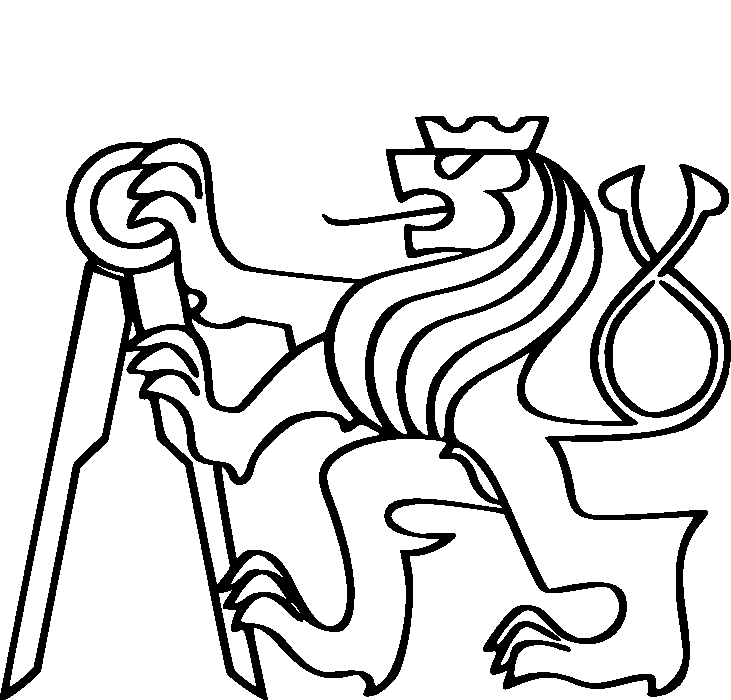
\includegraphics[scale=0.28]{../../_meta/cvut_standart.pdf}
\end{flushright}
\end{multicols}
\hrule
\vspace{0.5cm}

% ----------------------------------------------------------------------


% --- Tělo dokumentu ---------------------------------------------------

% Ocitovat markovu hlavičku
% Zeptat se na značky přístrojů

\setlength{\parindent}{0.5cm}

\part{Cejchování kompenzátorem}

\section{Pracovní úkoly}
\begin{enumerate}
  \item Pomocí kompenzátoru ocejchujte stupnici voltmetru (cejchujte v celém rozsahu stupnice). Pro 10 naměřených hodnot sestrojte kalibrační křivku a vyneste ji do grafu.
  \item Pomocí kompenzátoru ocejchujte stupnici miliampérmetru (cejchujte v celém rozsahu stupnice). Pro 10 naměřených hodnot sestrojte kalibrační křivku a vyneste ji do grafu.
\end{enumerate}

\section{Vypracování}

\subsection{Použité přístroje}
Miliampérmetr, voltmetr, 0-20V zdroj, 1,5V akumulátor, reostaty 115 $\Omega$ a 23200 $\Omega$, vodiče, odporový normál 100 $\Omega$, technický kompenzátor QTK Metra, Westonův normální článek, teploměr.

\subsection{Teoretický úvod}
\subsubsection{Kompenzátor}
Pro co nejpřesnější měření elektromotorického napětí stejnosměrných zdrojů je vhodné použít kompenzační metodu. Využívá se při ní faktu, že je snazší přesně určit, kdy je napětí v dané části obvodu nulové, než určovat jeho absolutní nenulovou velikost. Další výhodou kompenzátorů je, že nezatěžují zdroj proudem a nemění tak jeho napěťovou charakteristiku. 

Na obrázku \ref{fig:s_princip_kompenzatoru} je znázorněno principiální schéma zapojení kompenzátoru. Referenční napětí značíme $U$, neznámé pak $U_{x}$. Obvodem protéká proud podle toho jak moc se od sebe tyto dvě napětí liší. Velikost výchylky v takovém případě sledujeme na galvanometru $G$. Když nastavíme $U$ tak, aby se rovnalo $U_{x}$, nebude galvanometr ukazovat nic a říkáme, že je $U_{x}$ vykompenzováno napětím $U$. K měření využíváme kompenzátor METRA typu QTK po zkonzultování detailního návodu v dokumentu \cite{bib:pra_navody_o}.

Schéma zapojení kompenzátoru do obvodu je vidět na obrázku \ref{fig:s_zapojeni_kompenzatoru}. Písmenem $A$ je na něm vyznačen pomocný obvod, zatímco označení $B$ nese obvod měřený. Oba obvody jsou vzájemně provázány skrze potenciometr $R_{1}$. V momentu, kdy se nám podaří dostat jezdce do takové polohy, aby napětí na něm $U$ bylo rovno napětí měřeného zdroje $U_{m}$, přestane obvodem $B$ protékat proud a výchylka na galvanometru bude nulová. Proud v obvodu $A$ v tu chvíli přestane ovlivňovat obvod $B$ a vzhledem k vyrovnání obou napětí bude platit:

\begin{equation}
RI_{p} = U = U_{m},
\label{eq:e_kompenzator_1}
\end{equation}

kde $R$ je odpor na jezdci. Velikost proudu $I_p$ se určuje nepřímo, pomocí Westonova normálního článku, který zapojíme na místo napětí $U_{m}$, které chceme změřit. Pakliže vykompenzujeme napětí tohoto článku (označíme ho $U_{N}$, jeho odpor pak $R_N$), bude platit :

\begin{equation}
R_{N}I_{p} = U_{N}, \qquad U_{m} = \frac{R}{R_{N}}U_{N}
\label{eq:e_kompenzator_2}
\end{equation}

Musíme si však stále dávat pozor, aby se proud $I_{p}$ pokud možno vůbec neměnil. Pro napětí $U_{N}$ Westonova normálního článku platí vztah

\begin{equation}
U_n = U_{20} - 4.06 \cdot 10^{-5} (t-20) - 0.95 \cdot 10^{-6} (t-20)^2 + 1 \cdot 10 ^{-8} (t-20)^3 \ \unit{V},
\label{eq:e_weston_1}
\end{equation}

kde $U_{20} = 1,01865$ V jak se ostatně můžeme dočíst v dokumentu \cite{bib:pra_navody_o}, kde je Westonův článek popsán do větších detailů.


\begin{figure}[h!]
\centering
  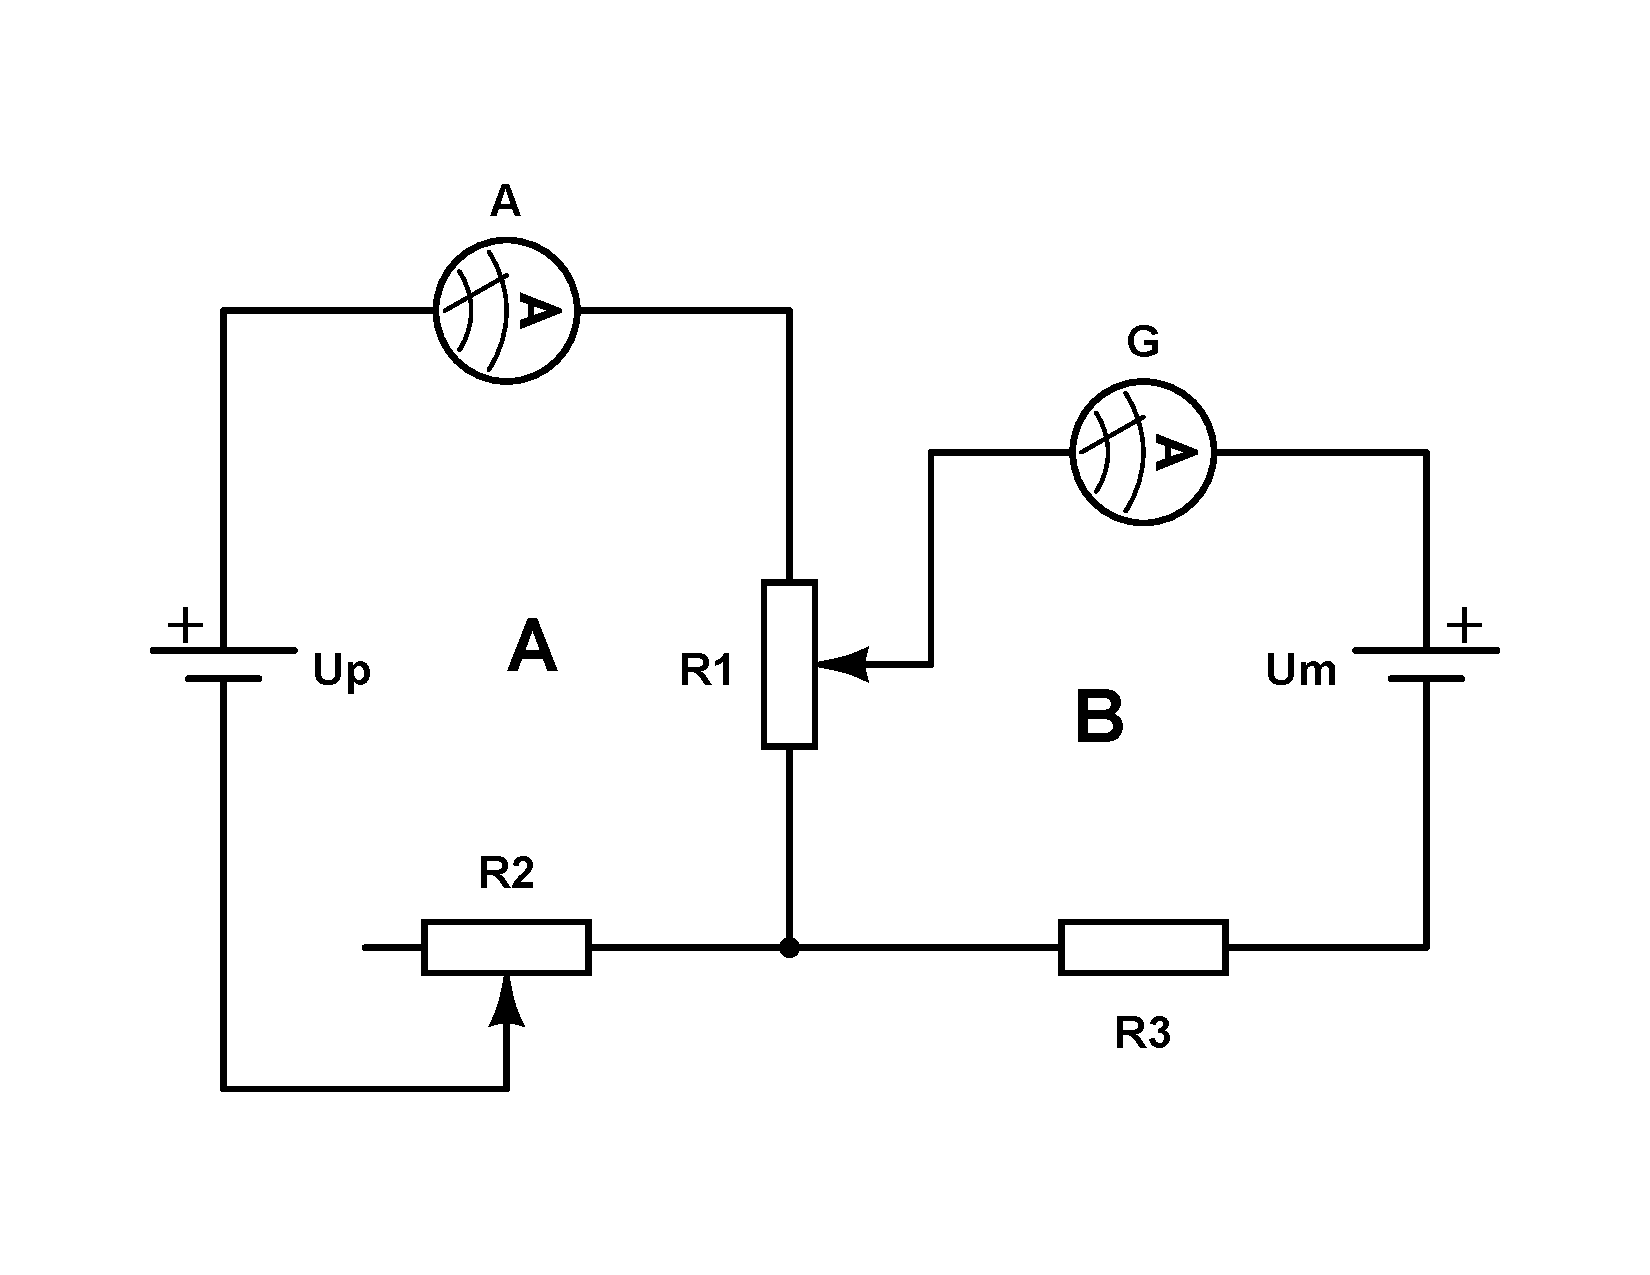
\includegraphics[scale=0.4, trim=0cm 3cm 0cm 3cm, clip=true]{att/7_s_zapojeni_kompenzatoru.pdf}
  \caption{Schéma zapojení kompenzátoru}
  \label{fig:s_zapojeni_kompenzatoru}
\end{figure}

\begin{figure}[h!]
\centering
  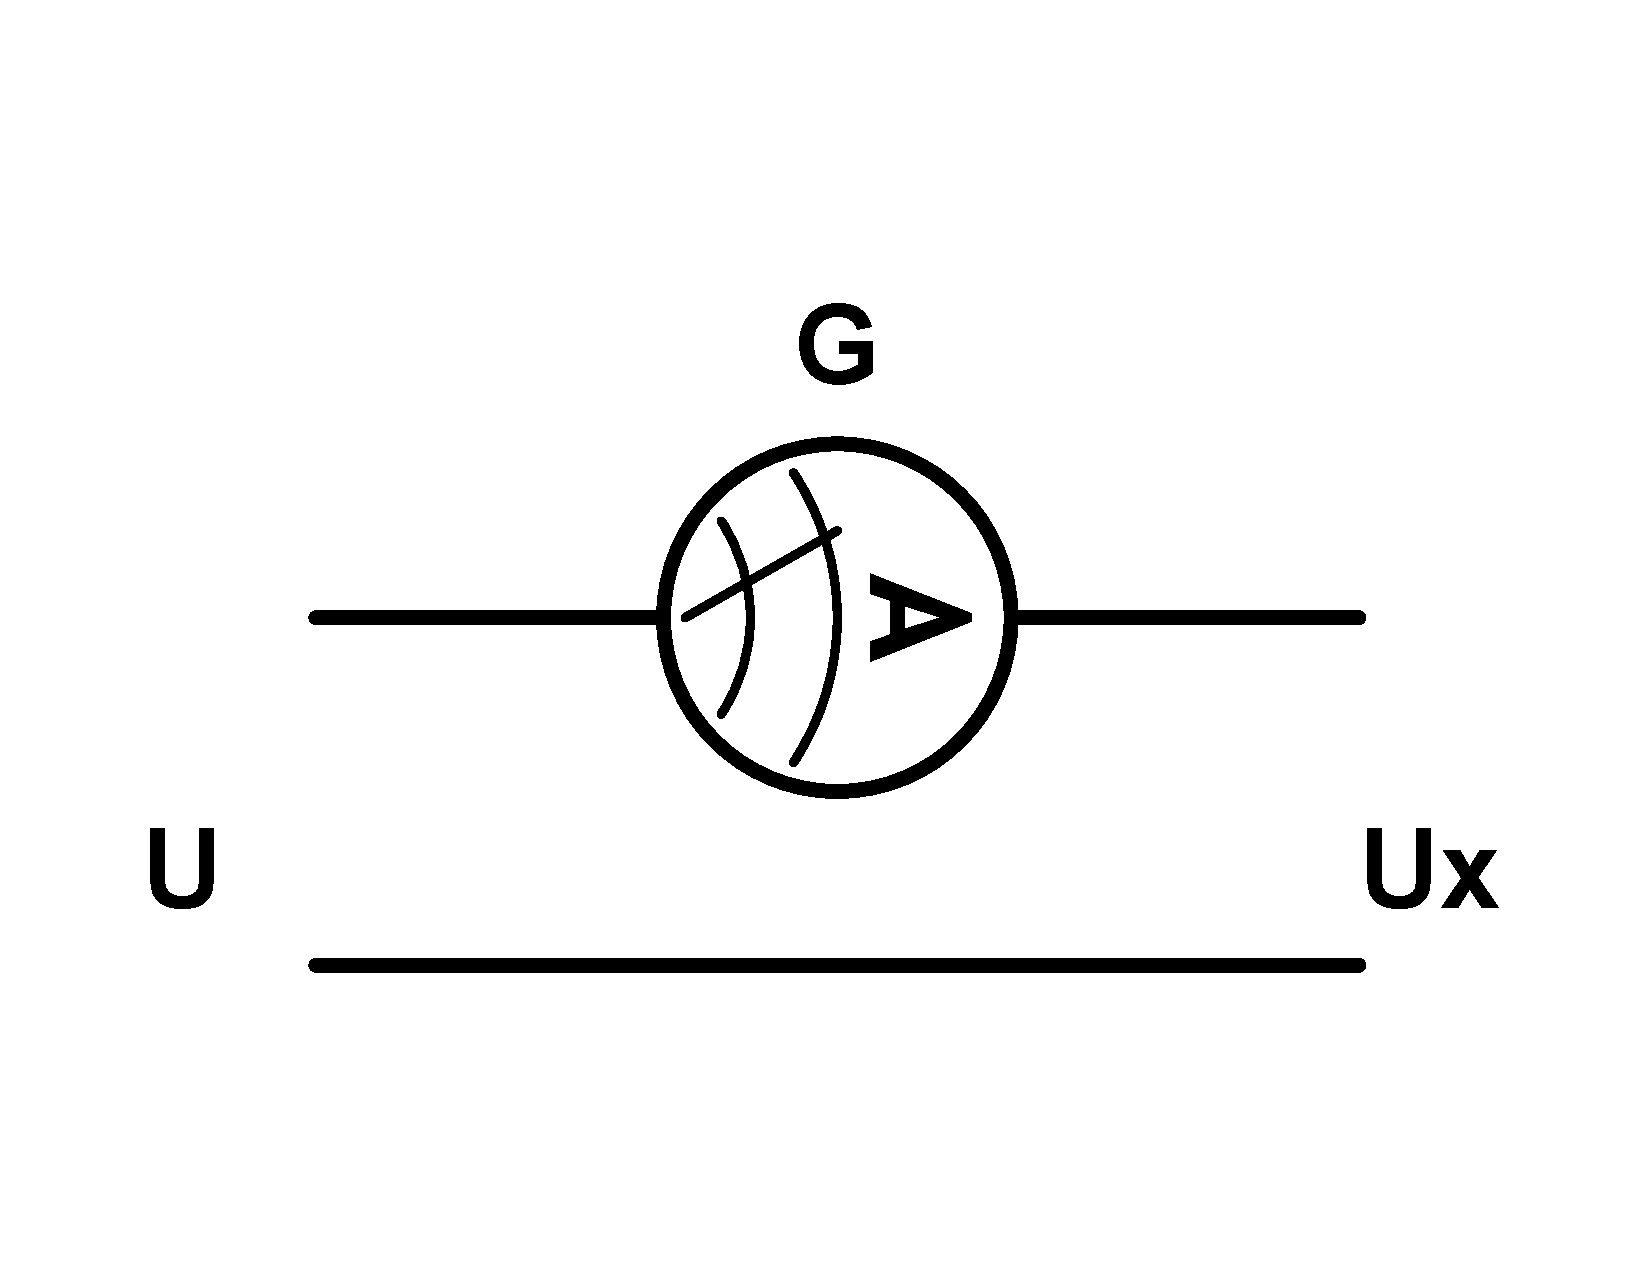
\includegraphics[scale=0.2, trim=0cm 5cm 0cm 5cm, clip=true]{att/7_s_princip_kompenzatoru.pdf}
  \caption{Principiální schéma zapojení kompenzátoru}
  \label{fig:s_princip_kompenzatoru}
\end{figure}

\subsubsection{Cejchování voltmetru}
Na obrázku \ref{fig:s_cejchovani_v} vidíme, že se cejchování provádí pomocí reostatu $R_{1}$, kterým vkládáme na svorky voltmetru $V$ různé stejnosměrné napětí, a kompenzátoru, pomocí kterého určíme jeho správnou hodnotu $U_{k}$. Tu následně porovnáme s hodnotou $U_{v}$ odečtenou z proměřovaného voltmetru.

\begin{figure}[h!]
\centering
  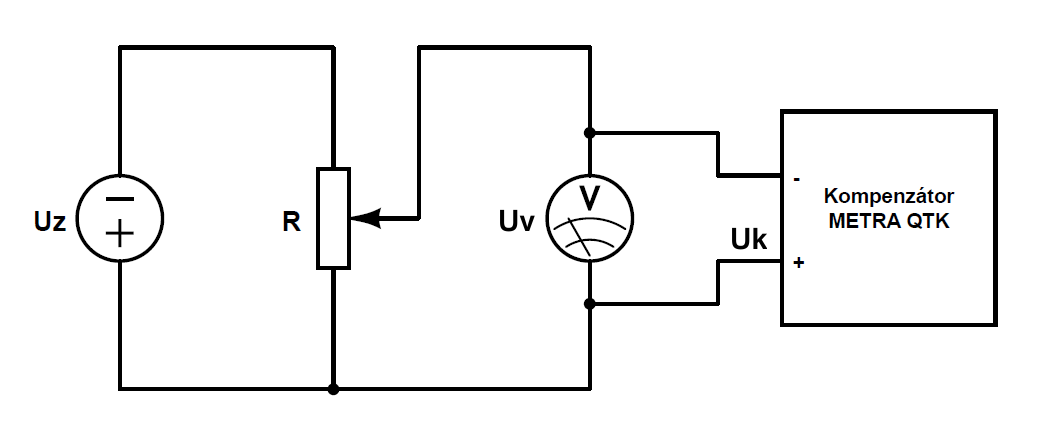
\includegraphics[scale=0.4]{att/7_s_cejchovani_v.png}
  \caption{Schéma zapojení při cejchování voltmetru \cite{bib:repo}.}
  \label{fig:s_cejchovani_v}
\end{figure}

\subsubsection{Cejchování miliampérmetru}
Zapojení pro tento úkol je znázorněno na obrázku \ref{fig:s_cejchovani_a}. Přes změny na reostatu $R$ měníme proud $I_{a}$, který prochází odporovým normálem $R_{n}$. Na něm vzniká úbytek napětí $U_{k}$ a to změříme opět za použití kompenzátoru. Vlastní hodnotu proudu pak určíme podle rovnice \ref{eq:e_cejch_mil} a porovnáme ji s hodnotou odečtenou z miliampérmetru $A$.

\begin{equation}
I_{a}=\frac{U_{k}}{R_{n}}
\label{eq:e_cejch_mil}
\end{equation}

\begin{figure}[h!]
\centering
  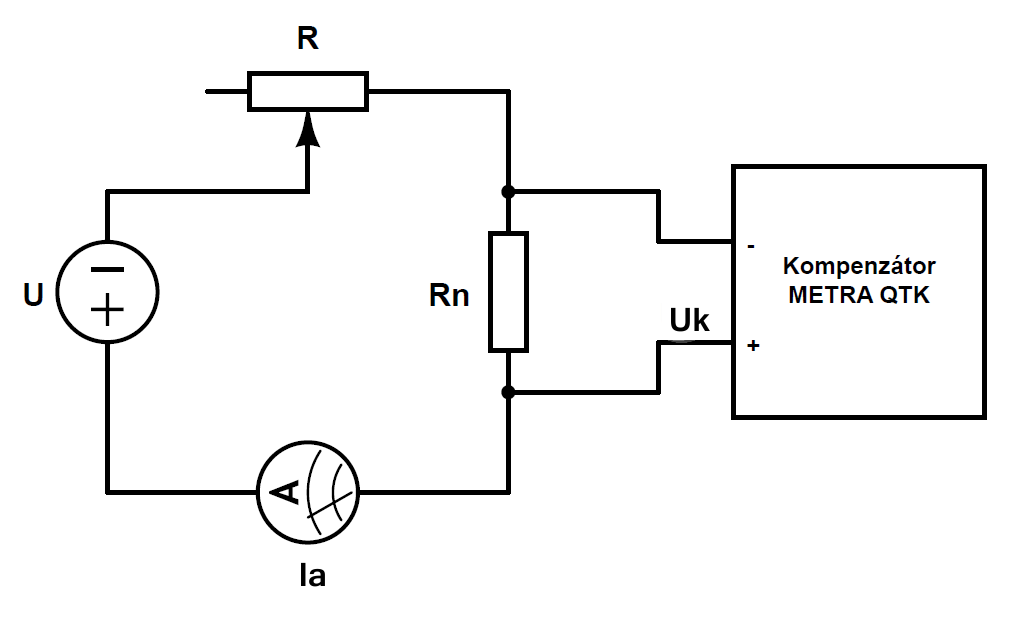
\includegraphics[scale=0.4]{att/7_s_cejchovani_a.png}
  \caption{Schéma zapojení při cejchování miliampérmetru \cite{bib:repo}.}
  \label{fig:s_cejchovani_a}
\end{figure}

\subsection{Postup měření}
\subsubsection{Kompenzátor}
První věc, kterou jsme museli začít, byla kalibrace kompenzátoru pomocí Westonova normálního článku. Tuto kalibraci jsme během experimentu provedli vícekrát vzhledem ke změně teploty v místnosti (viz rovnice \ref{eq:e_weston_1}). Celý postup jsme museli provádět s maximální opatrností, jelikož je Westonův článek velmi křehký. Nejdříve jsme napětí z něj přivedli na svorky označené $U_{N}$, pak na kompenzátoru nastavili co nejpřesněji hodnotu napětí článku pro danou teplotu a zapnuli vnitřní zdroj. Následně bylo zapotřebí nastavit kompenzátor tak, aby byla výchylka galvanometru nulová a pomocný proud měl hodnotu přesně 1 mA. Teplota v místnosti během měření postupně rostla z 18 $^\circ$C na 22 $^\circ$C.

Se zkalibrovaným kompenzátorem pak probíhá měření následovně:
\begin{enumerate}
  \item Nastavíme kompenzátor tak, aby měřil na svorkách $U_{x}$ ve vhodném rozsahu.
  \item Napětí, které chceme změřit připojíme k těmto svorkám a nastavíme předpokládanou hodnotu napětí.
  \item Zapneme vnitřní zdroj a rychlým vychýlením páčky do směru \emph{hrubě} zjistíme, jak velká je odchylka na galvanometru a jakým směrem.
  \item Podle této výchylky vhodně upravíme napětí vnitřního zdroje kompenzátoru.
  \item V momentu, kdy bude výchylka téměř nepozorovatelná, začneme páčky vychylovat ve směru \emph{jemně} (na druhou stranu).
  \item Jemným upravováním napětí vnitřního zdroje kompenzátoru opět dosáhneme nulové výchylky.
  \item Napětí nastavené nastavené na kompenzátoru vynásobíme podle aktuálního rozsahu a zaznamenáme. 
\end{enumerate}

\subsubsection{Cejchování voltmetru}
Schéma zapojení pro tuto část postupu je znázorněno na obrázku \ref{fig:s_cejchovani_v}. Zdroj $U_{z}$ měl v našem případě stejnosměrné napětí 10 V a kompenzátor jsme nastavili na rozsah 15 V. Přes reostat $R$ 115 $\Omega$ jsme nastavovali napětí $U_{v}$ na svorkách voltmetru a to po zaznamenání porovnávali s hodnotou napětí $U_{k}$, kterou ukazoval kompenzátor. Podle získaných hodnot obou napětí jsme pak sestrojili kalibrační křivku. 

\subsubsection{Cejchování miliampérmetru}
Obvod jsme zapojili dle obrázku \ref{fig:s_cejchovani_a}, za zdroj $U$ nám sloužil akumulátor o hodnotě napětí $1,5$ V a kompenzátor jsme nastavili na rozsah $1500$ mV. Ke změně napětí na odporovém normálu $U_k$ (měřeného kompenzátorem) slouží reostat $R$ $23200\ \Omega$. Pomocí tohoto napětí a rovnice \ref{eq:e_cejch_mil} pak dopočítáme proud $I_{k}$, který porovnáme s proudem $I_a$ odečteným na cejchovaném miliampérmetru. Podle získaných hodnot obou proudů sestrojíme kalibrační křivku.

\subsection{Naměřené hodnoty}

Naměřené hodnoty jsou vyneseny v tabulkách \ref{tab:cejchovani_voltmetru} a \ref{tab:cejchovani_ampermetru}. V grafech \ref{fig:g_cejchovani_a} a \ref{fig:g_cejchovani_v} vidíme naměřené hodnoty při cejchování obou přístrojů, kalibrační křivky každého z nich pak v grafech \ref{fig:g_cejchovani_v_kalib} a \ref{fig:g_cejchovani_a_kalib}.

\begin{table}[h]
\begin{center}
\begin{tabular}{|r|r|r|r|}
\hline
   $U_{k}$ [V] & $U_{v}$ [V] & $\Delta U$ [V] & $ \Delta U_{r} $ [\%]\\\hline
   
   $0,987$&$1,0$&$-0,013$&$1,30$\\\hline
   $1,971$&$2,0$&$-0,029$&$1,45$\\\hline
   $2,966$&$3,0$&$-0,034$&$1,13$\\\hline
   $3,904$&$4,0$&$-0,096$&$2,40$\\\hline
   $4,922$&$5,0$&$-0,078$&$1,56$\\\hline
   $5,905$&$6,0$&$-0,095$&$1,58$\\\hline
   $6,894$&$7,0$&$-0,106$&$1,51$\\\hline
   $7,873$&$8,0$&$-0,127$&$1,59$\\\hline
   $8,816$&$9,0$&$-0,184$&$2,04$\\\hline
   $9,753$&$10,0$&$-0,247$&$2,47$\\\hline

\end{tabular}
\caption{Cejchování voltmetru. $U_{k}$ je hodnota napětí změřená kompenzátorem, $U_{v}$ hodnota odečtená na voltmetru, $\Delta U $ rozdíl obou napětí, $ \Delta U_{r} $ relativní rozdíl těchto napětí v procentech (vztaženo k $U_{v}$).}
\label{tab:cejchovani_voltmetru}
\end{center}
\end{table}

\begin{figure}[p]
\begin{center}
    \vspace*{-1cm}
	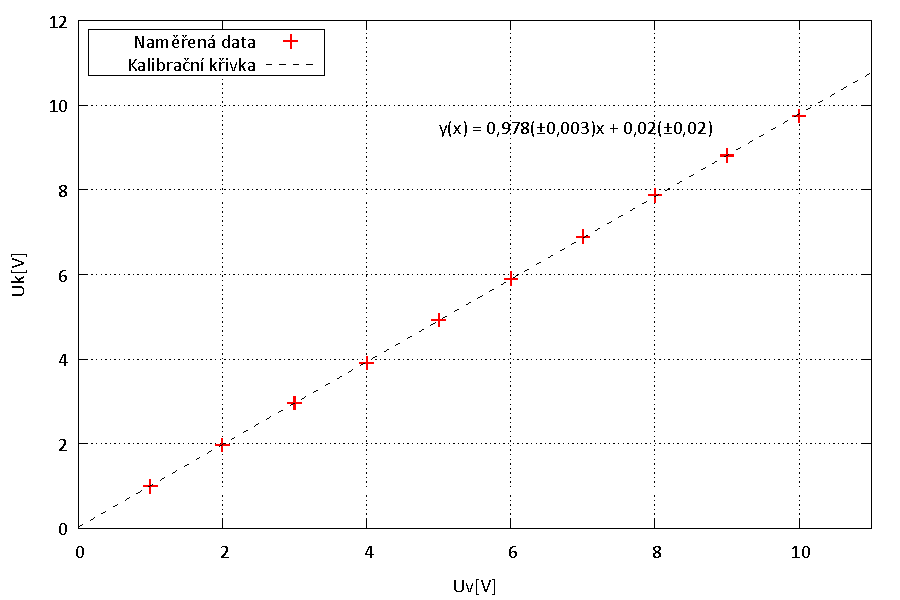
\includegraphics[width=\linewidth]{../gnuplot/7_kompenzator_cejvolt_out.pdf}
    \vspace*{-1cm}
	\caption{Graf hodnot naměřených při cejchování voltmetru. Výsledky jsme proložili lineární regresí, které využíváme pro diskusi výsledků v druhé části.}
	\label{fig:g_cejchovani_v}
\end{center}
\end{figure}

\begin{figure}[p]
\begin{center}
    \vspace*{-1cm}
    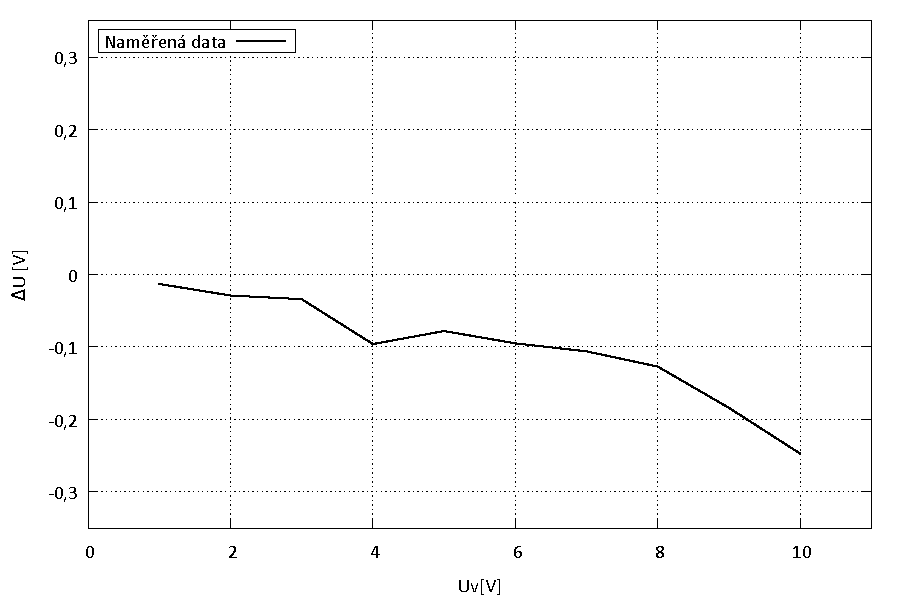
\includegraphics[width=\linewidth]{../gnuplot/7_kompenzator_cejvolt_kalib_out.pdf}
    \vspace*{-1cm}    
	\caption{Graf kalibrační křivky voltmetru.}
	\label{fig:g_cejchovani_v_kalib}
\end{center}
\end{figure}

\begin{table}[h]
\begin{center}
\begin{tabular}{|r|r|r|r|r|}
\hline
   $U_{k}$ [mV] & $I_{k}$ [mA] & $I_{a}$ [mA] & $\Delta I$ [mA] & $ \Delta I_{r} $ [\%]\\\hline
   
   $7,0$  & $0,070$ & $0,080$ & $-0,010$ & $12,50$\\ \hline
   $14,3$ & $0,143$ & $0,160$ & $-0,017$ & $10,63$\\ \hline
   $22,2$ & $0,222$ & $0,240$ & $-0,018$ &  $7,50$\\ \hline
   $32,1$ & $0,321$ & $0,320$ & $0,001$  &  $0,31$\\ \hline
   $37,9$ & $0,379$ & $0,400$ & $-0,021$ &  $5,25$\\ \hline
   $45,9$ & $0,459$ & $0,480$ & $-0,021$ &  $4,38$\\ \hline
   $54,0$ & $0,540$ & $0,560$ & $-0,020$ &  $3,57$\\ \hline
   $58,9$ & $0,589$ & $0,620$ & $-0,031$ &  $5,00$\\ \hline
   $67,4$ & $0,674$ & $0,700$ & $-0,026$ &  $3,71$\\ \hline
   $75,3$ & $0,753$ & $0,780$ & $-0,027$ &  $3,46$\\ \hline

\end{tabular}
\caption{Cejchování ampérmetru. $U_{k}$ je hodnota napětí změřená kompenzátorem, $I_{k}$ z ní dopočítaná hodnota proudu, $I_{a}$ hodnota odečtená na miliampérmetru, $\Delta I $ rozdíl obou proudů, $ \Delta I_{r} $ relativní rozdíl těchto proudů v procentech (vztaženo k $I_{a}$).}
\label{tab:cejchovani_ampermetru}
\end{center}
\end{table}

\begin{figure}[p]
\begin{center}
	\vspace*{-1cm}
	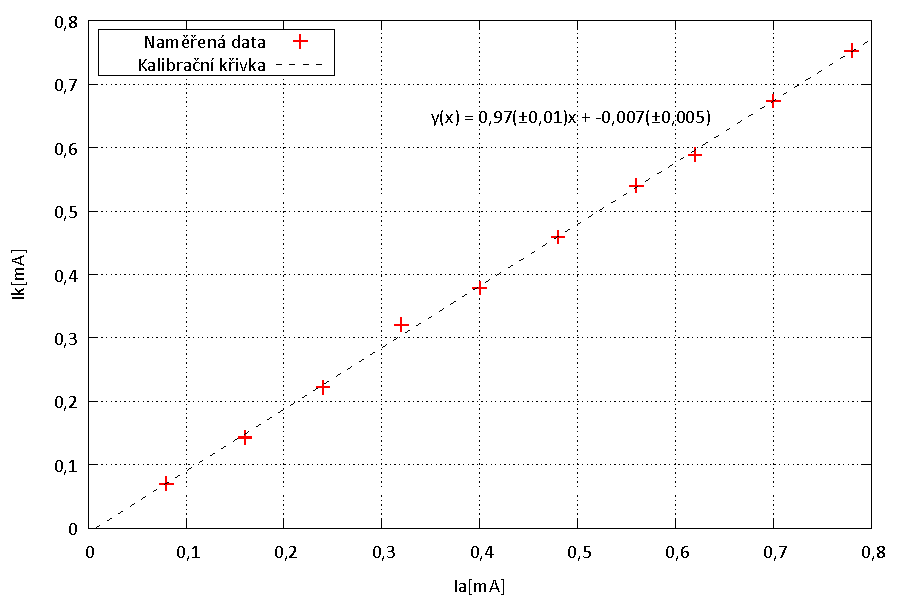
\includegraphics[width=\linewidth]{../gnuplot/7_kompenzator_cejamper_out.pdf}
	\vspace*{-1cm}
	\caption{Graf hodnot naměřených při cejchování ampérmetru. Výsledky jsme opět proložili lineární regresí.}
	\label{fig:g_cejchovani_a}
\end{center}
\end{figure}

\begin{figure}[p]
\begin{center}
	\vspace*{-1cm}
	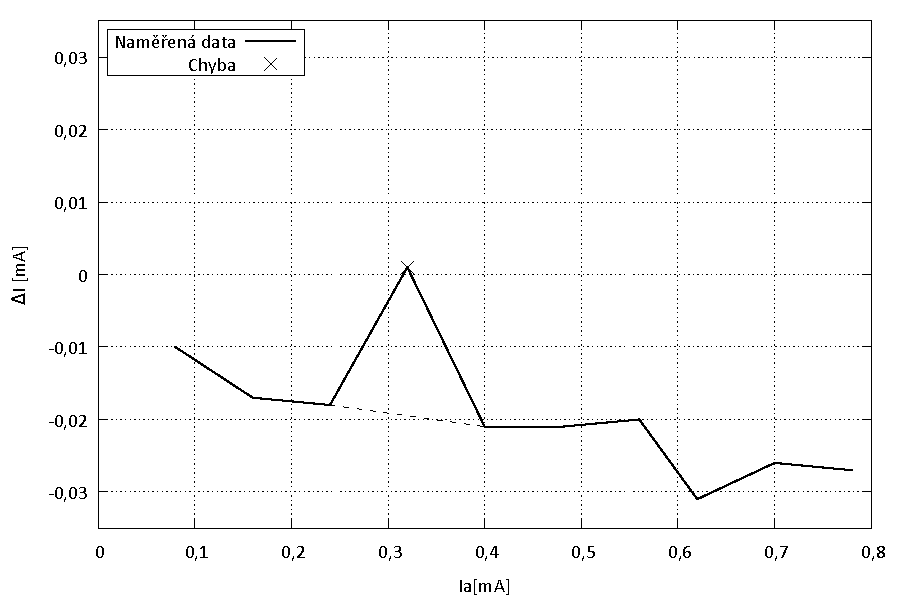
\includegraphics[width=\linewidth]{../gnuplot/7_kompenzator_cejamper_kalib_out.pdf}
	\vspace*{-1cm}
	\caption{Graf kalibrační křivky voltmetru. U jednoho z bodů se může jednat o chybu, přerušovaná čára naznačuje jak by kalibrační křivka vypadala v případě, že bychom ho z uvažovaných hodnot vyřadili.}
	\label{fig:g_cejchovani_a_kalib}
\end{center}
\end{figure}

\subsection{Diskuse}
\subsubsection{Cejchování voltmetru}
Velikost odchylek dosahovala maximálně desetin voltu, což odpovídá jednotkám procent měřeného napětí. Pro toto měření jsme využívali na kompenzátoru rozsahu 15 V, což vedlo k menší přesnosti měření, vzhledem k tomu, že se galvanometr v blízkosti přesné hodnoty vychyloval jen velmi málo a bylo ji tak těžší dobře určit. 

\subsubsection{Cejchování miliampérmetru}
Velikost odchylek dosahovala maximálně desetin miliampéru, což při měření nižších hodnot proudu odpovídá až 12,5 procentům měřeného proudu, zatímco u vyšších hodnot jde o méně než 4 procenta. Potvrdilo se tedy, že větší přesnosti při měření s ampérmetrem dosáhneme, pokud se na něm hodnoty pohybují v poslední třetině stupnice. Jedna z hodnot je znatelně odlišná od ostatních a je možné, že se jedná o chybu měření. Na kalibrační křivce je vyznačeno, jak by vypadala v případě, že bychom brali bod jako chybný. Pro proložení lineární regresí jsme však brali měření jako správné. Pro další závěry by bylo potřeba měření provést vícekrát a s větší hustotou bodů.

\section{Závěr}
Pomocí kompenzátoru METRA typu QTK jsme ocejchovali stupnici miliampérmetru a voltmetru v celém rozsahu a pro 10 naměřených hodnot jsme sestrojili a vynesli do grafu kalibrační křivku. Naměřené hodnoty jsme proložili lineární regresí, které využijeme pro diskusi v druhé části. 


\section {Použitá literatura}
% --- Literatura a reference -------------------------------------------

\begin{thebibliography}{9}
\bibitem{bib:pra_navod_uloha} Kolektiv KF, \emph{Návod k úloze: Rozšíření rozsahu Miliampérmetru a voltmetru. Cejchování kompenzátorem.} [Online], [cit. \today] \newline 
http://praktikum.fjfi.cvut.cz/pluginfile.php/119/mod\_resource/content/6/07rozsireni\_v1.pdf

\bibitem{bib:repo} Kolektiv autorů, \emph{Repozitář zdrojů k praktiku} [Online], podle \cite{bib:pra_navod_uloha} [cit. \today] \newline https://github.com/roesel/praktika

\bibitem{bib:pra_navody_o} Kolektiv KF, \emph{Návody k přístrojům} [Online], [cit. \today] \newline http://praktikum.fjfi.cvut.cz/documents/chybynav/navody-o.pdf
\end{thebibliography}

% ----------------------------------------------------------------------


\part{Rozšíření rozsahu miliampérmetru a voltmetru}

\section{Pracovní úkoly}
\begin{enumerate}
  \item V přípravě odvoďte vztah pro rozšíření rozsahu voltmetru $n$-krát.
  \item Rozšiřte rozsah miliampérmetru dvakrát a určete jeho vnitřní odpor. Měření proveďte pro 10 různých nastavení obvodu, t.j. pro 10 různých proudů.
  \item Rozšiřte rozsah voltmetru dvakrát a určete jeho vnitřní odpor. Měření proveďte pro 10 různých nastavení obvodu, t.j. pro 10 různých napětí.
  \item Při zpracování výsledků z měření vnitřních odporů vezměte v úvahu výsledky získané cejchováním stupnic voltmetru a miliampérmetru a proveďte korekci naměřených hodnot. Diskutujte rozdíl mezi výsledkem získaným bez korekce a s korekcí.
\end{enumerate}

\section{Vypracování}

\subsection{Použité přístroje}
Miliampérmetr, voltmetr, 0-20V zdroj, odporová dekáda, reostaty 115 $\Omega$ a 23200 $\Omega$, dva vypínače, vodiče.

\subsection{Teoretický úvod}
Chceme-li měřit proud či napětí, jsme vždy omezováni rozsahem stupnice daného aparátu a hodí se nám ho rozšířit nejen pro zabránění přetížení přístroje. Toho dosáhneme pomocí přídavného rezistoru, jehož hodnota závisí na tom, jaké změny rozsahu chceme dosáhnout a jakým vnitřním odporem disponuje náš přístroj. 

\subsubsection{Rozšíření rozsahu miliampérmetru}
Měříme-li vyšší proudy, než na které nám stačí stupnice, využíváme tzv. \emph{bočníku} - odporu o konkrétní hodnotě, který zapojíme paralelně k ampérmetru tak jako na obrázku \ref{fig:s_rozsah_a}.   

\begin{figure}[h!]
\centering
  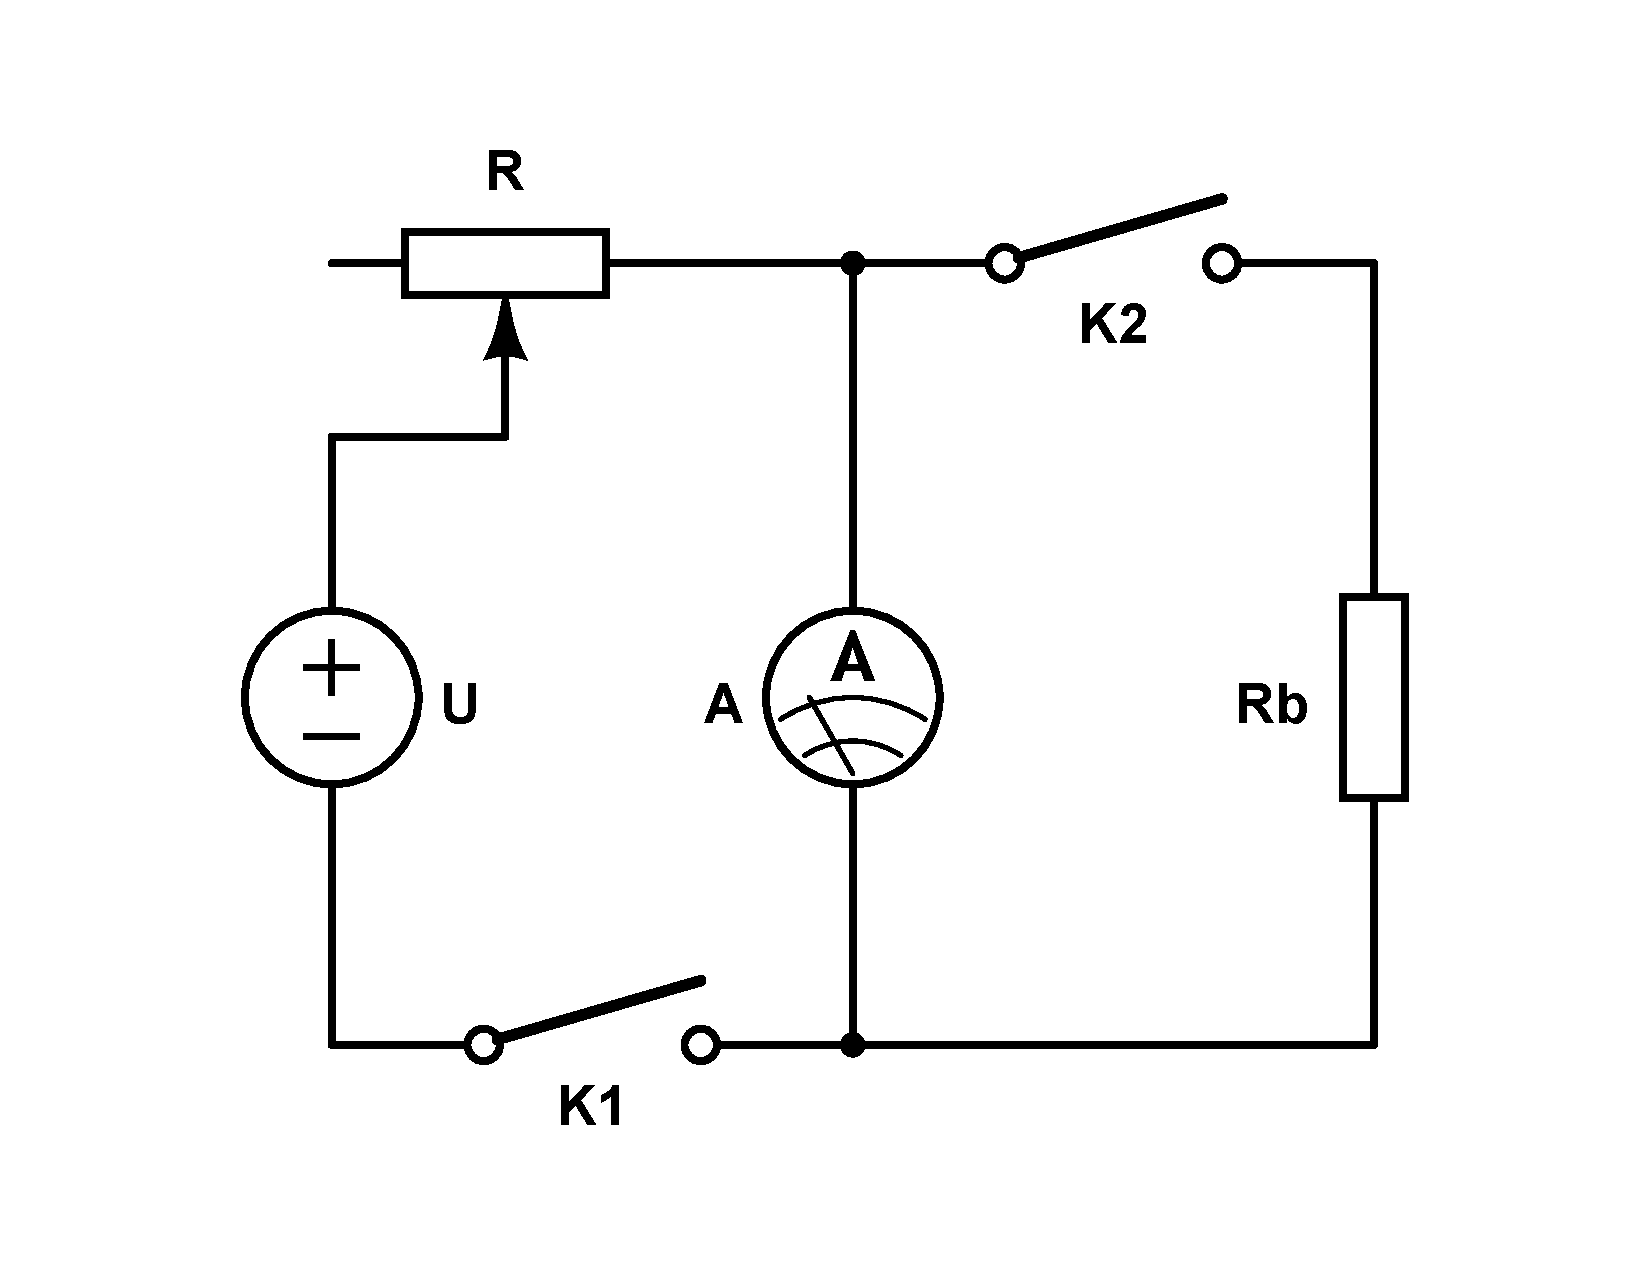
\includegraphics[scale=0.4, trim=0cm 2cm 0cm 2cm, clip=true]{att/7_s_rozsah_a.pdf}
  \caption{Schéma zapojení při rozšiřování rozsahu miliampérmetru  \cite{bib:repo_2}.}
  \label{fig:s_rozsah_a}
\end{figure}

Zajímá nás, jaká je hodnota \emph{bočníku} $R_{b}.$ K dispozici máme dvě nastavení obvodu. Bude-li klíč $K_{2}$ vypnutý, poteče ampérmetrem proud $I_{1}$. Zapneme-li klíč $K_{2}$, bude ampérmetrem procházet proud $I_{2}$ a pro rozšíření rozsahu $n$-krát bude platit

\begin{equation} 
\frac{I_1}{I_2} = n.
\label{eq:odovozeni_a_rozsah_podminka_n}
\end{equation}

Vypneme-li klíč $K_{2}$, bude proud protékající oběma ampérmetry stejný a bude platit

\begin{equation} 
\frac{U}{R+R_{0}} = I_{1},
\label{eq:odovozeni_a_rozsah_1}
\end{equation}
 
kde $R_{0}$ je vnitřní odpor ampérmetru $A$ a $R$ je vnitřní odpor zdroje. Dále budou při dostatečně velkém odporu $R$ platit následující vztahy 

\begin{equation} 
\frac{I_{2}}{I_{b}}=\frac{R_{b}}{R_{0}}, \qquad  I_1 = I_2 + I_b, \qquad  \frac{I_{b}}{I_{2}}=\frac{I_{1}}{I_{2}}-1 = n-1,
\label{eq:odovozeni_a_rozsah_2}
\end{equation}

ze kterých získáváme pro odpor \emph{bočníku} $R_{b}$ 

\begin{equation} 
R_{b} = \frac{I_{2}}{I_{b}}R_{0} = \frac{R_{0}}{\frac{I_{b}}{I_{2}}} = \frac{R_{0}}{n-1} .
\label{eq:odovozeni_a_rozsah_3}
\end{equation}

\subsubsection{Rozšíření rozsahu voltmetru}
Měříme-li vyšší napětí, než na které nám stačí stupnice, využíváme tzv. \emph{předřadného odporu} o konkrétní hodnotě, který zapojíme sériově s voltmetrem tak jako na obrázku \ref{fig:s_rozsah_v}.   

\begin{figure}[h!]
\centering
  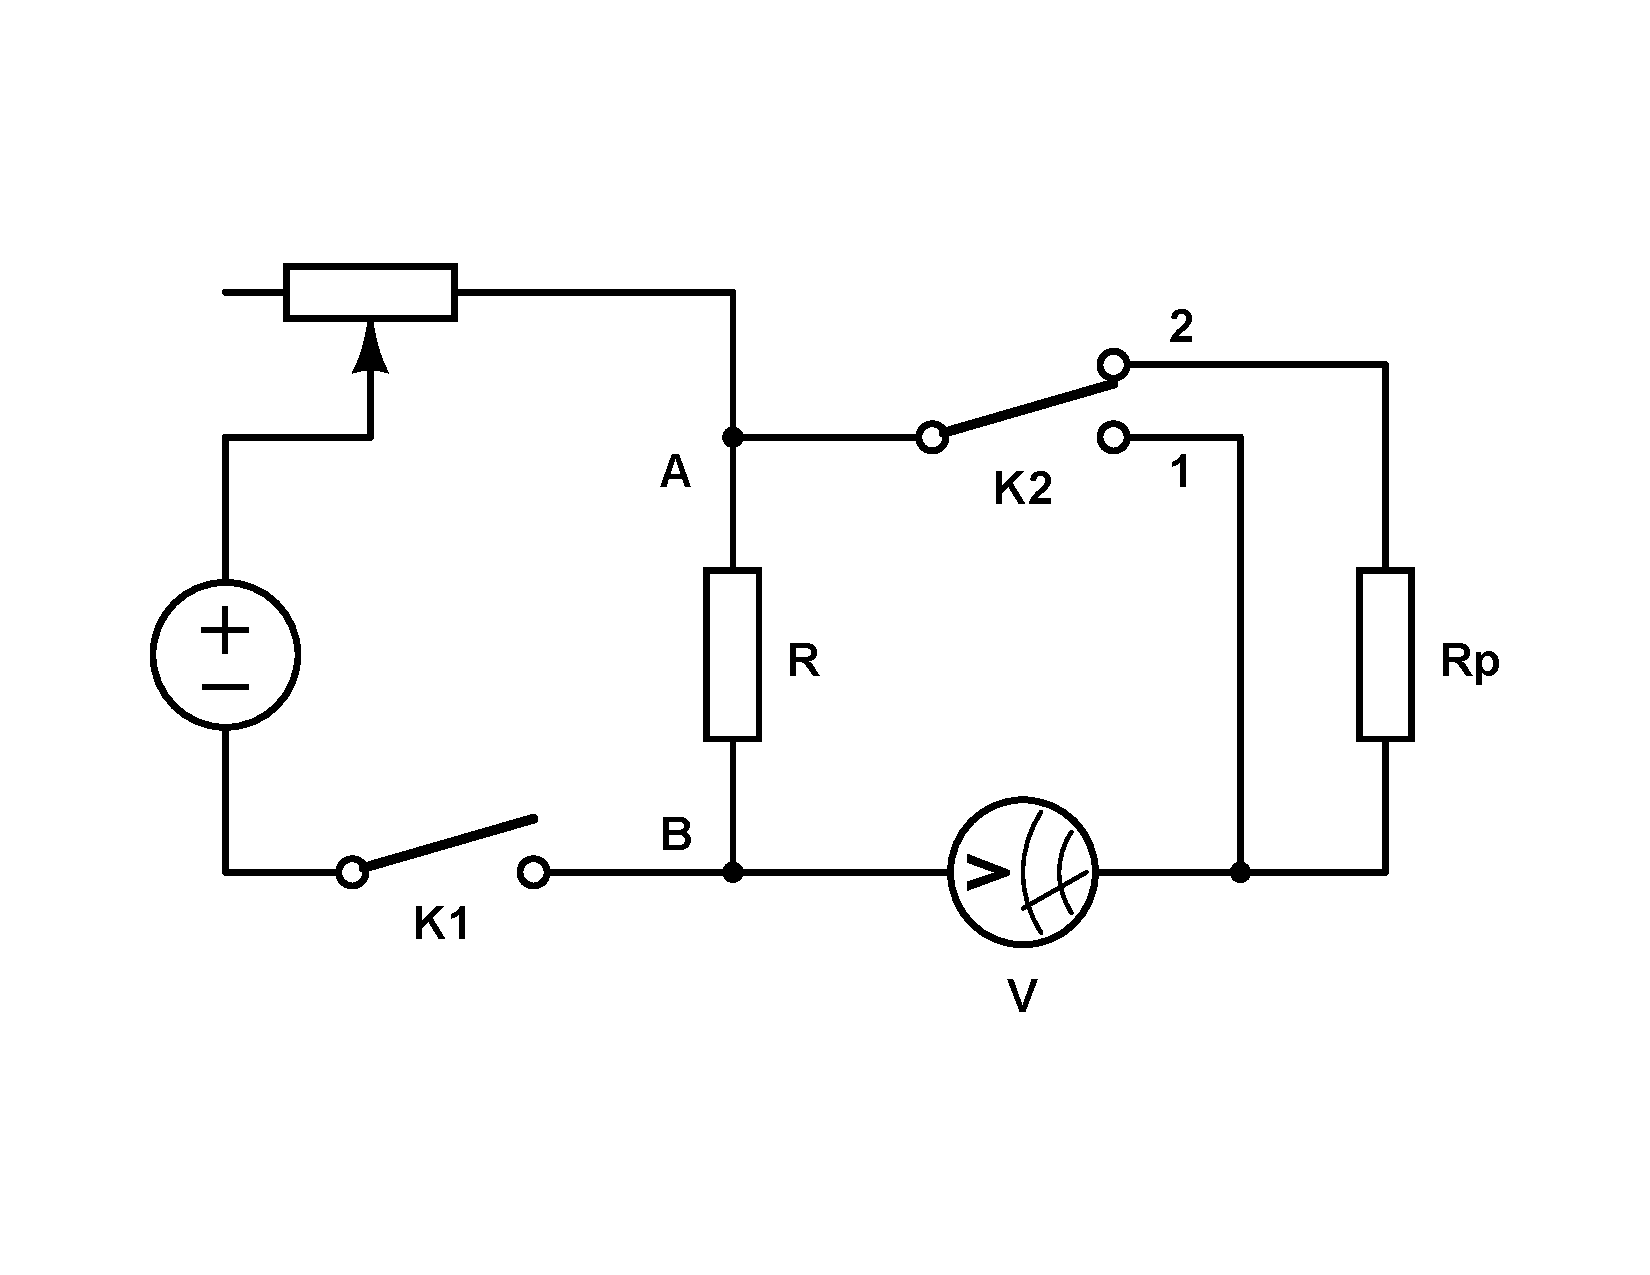
\includegraphics[scale=0.4, trim=0cm 2cm 0cm 2cm, clip=true]{att/7_s_rozsah_v.pdf}
  \caption{Schéma zapojení při rozšiřování rozsahu voltmetru \cite{bib:repo_2}.}
  \label{fig:s_rozsah_v}
\end{figure}
  
Zajímá nás, jaká je hodnota \emph{předřadného odporu} $R_{p}.$ K dispozici máme opět dvě nastavení obvodu. Bude-li klíč $K_{2}$ v poloze 1, poteče voltmetrem proud $I_{v}$ a podle Ohmova zákona bude za předpokladu dostatečně malého odporu $R$ platit

\begin{equation} 
I_{v} = \frac{U_{v}}{R_{0}} = \frac{U}{R_{0}+R_{p}} = \frac{U - U_{v}}{R_{p}},
\label{eq:odvozeni_v_rozsah_1}
\end{equation}

kde $U$ je napětí mezi body $A$ a $B$, $U_{v}$ napětí na voltmetru a $R_{0}$ jeho vnitřní odpor. Chceme-li rozšířit rozsah voltmetru $n$-krát, musí zároveň platit

\begin{equation} 
\frac{U}{U_{v}} = n
\label{eq:odvozeni_v_rozsah_n}
\end{equation}

a odtud dostáváme finální hodnotu \emph{předřadného odporu} $Rp$ jako

\begin{equation} 
R_{p} = \frac{R_{0}(U-U_{v})}{U_{v}} = R_{0}(n-1).
\label{eq:odvozeni_v_rozsah_2}
\end{equation}

\subsubsection{Statistické zpracování}

Pro statistické zpracování využíváme aritmetického průměru:

\begin{equation} \label{eq:aritmeticky_prumer}
\overline{x} = \frac{1}{n}\sum\limits_{i=1}^{n}x_i
\end{equation}

jehož chybu spočítáme jako 

\begin{equation} \label{eq:chyba_aritmetickeho_prumeru}
\sigma_0 = \sqrt{\frac{1}{n(n-1)} \sum\limits_{i=1}^{n}\left( x_i - \overline{x} \right)^2 },
\end{equation}

kde $ x_i $ jsou jednotlivé naměřené hodnoty, $ n $ je počet měření, $ \overline{x} $ aritmetický průměr a $ \sigma_0 $ jeho chyba \cite{bib:pra_chyby_o_2}.

\subsection{Postup měření}

\subsubsection{Rozšíření rozsahu miliampérmetru}
Schéma zapojení pro tuto část postupu je znázorněno na obrázku \ref{fig:s_rozsah_a}. Zdroj měl v našem případě stejnosměrné napětí 10 V a jako rezistor $R$ nám sloužil reostat 23200 $\Omega$ jehož jezdec dovoloval v krajní poloze dosáhnout téměř přesně maxima stupnice miliampérmetru. Jako bočník jsme použili odporovou dekádu a postupovali pro každou hodnotu odporu $R$ následovně:
\begin{enumerate}
	\item S vypnutým vypínačem $K_{2}$ nastavíme na reostatu takový odpor, aby byla ručička ampérmetru za první třetinou stupnice na dobře čitelné hodnotě $I_{1}$, kterou zaznamenáme.
	\item Vypínač $K_{2}$ zapneme a na dekádě nastavíme takový odpor, aby miliampérmetr ukazoval proud $I_{2}$ o velikosti jedné poloviny předchozí hodnoty $I_{1}$. Odpor nastavený na dekádě zaznamenáme.
	\item Tento postup opakujeme pro 10 různých hodnot proudu posunem jezdce na reostatu. 	
\end{enumerate}

\subsubsection{Rozšíření rozsahu voltmetru}
Obvod jsme zapojili dle obrázku \ref{fig:s_rozsah_v}, zdroj měl v našem případě stejnosměrné napětí 10 V a jako rezistor $R$ jsme opět použili reostat 115 $\Omega$. Jako předřadný odpor jsme použili odporovou dekádu a postupovali pro každou hodnotu odporu $R$ následovně:
\begin{enumerate}
	\item S vypínačem $K_{2}$ v poloze 1 nastavíme na reostatu takový odpor, aby byla ručička voltmetru za první třetinou stupnice na dobře čitelné hodnotě $U_{1}$, kterou zaznamenáme.
	\item Vypínač $K_{2}$ přepneme do polohy 2 a na dekádě nastavíme takový odpor, aby voltmetr ukazoval napětí $U_{2}$ o velikosti jedné poloviny předchozí hodnoty $U_{1}$. Odpor nastavený na dekádě zaznamenáme.
	\item Tento postup opakujeme pro 10 různých hodnot napětí posunem jezdce na reostatu. 	
\end{enumerate}

\subsection{Naměřené hodnoty}
Naměřené hodnoty jsou v tabulkách \ref{tab:rozsirovani_ampermetru} a \ref{tab:rozsirovani_voltmetru}.

\begin{table}[h]
\catcode`\-=12 % HAX na enable cline v českym bable
\begin{center}
\begin{tabular}{|r|r|r|r|r|r|r|}
\hline
      $I_1 [mA]$ & $I_2 [mA]$ & $I_{1k} [mA]$ & $I_{2k} [mA]$ & $n_k [-]$ & $R_b [\Omega]$ & $R_{0k} [\Omega]$\\ \hline
      $0,80$ & $0,40$ & $0,77$ & $0,38$ & $2,0184$ & $102,6$ & $104,5$\\ \hline
      $0,82$ & $0,41$ & $0,79$ & $0,39$ & $2,0179$ & $104,4$ & $106,3$\\ \hline
      $0,84$ & $0,42$ & $0,81$ & $0,40$ & $2,0175$ & $103,2$ & $105,0$\\ \hline
      $0,86$ & $0,43$ & $0,83$ & $0,41$ & $2,0171$ & $105,6$ & $107,4$\\ \hline
      $0,88$ & $0,44$ & $0,85$ & $0,42$ & $2,0167$ & $106,5$ & $108,3$\\ \hline
      $0,90$ & $0,45$ & $0,87$ & $0,43$ & $2,0163$ & $104,8$ & $106,5$\\ \hline
      $0,92$ & $0,46$ & $0,89$ & $0,44$ & $2,0159$ & $105,9$ & $107,6$\\ \hline
      $0,94$ & $0,47$ & $0,90$ & $0,45$ & $2,0156$ & $106,3$ & $108,0$\\ \hline
      $0,96$ & $0,48$ & $0,92$ & $0,46$ & $2,0153$ & $104,5$ & $106,1$\\ \hline
      $0,98$ & $0,49$ & $0,94$ & $0,47$ & $2,0149$ & $106,2$ & $107,8$\\ \hline
      
      \multicolumn{2}{r|}{} & \multicolumn{3}{|r|}{Výsledné hodnoty \cite{bib:pra_chyby_o_2}:}  & $105,0 \pm 0,4$  & $106,7 \pm 0,4$ \\ 
      \cline{3-7} % pozor, cline vyžaduje hack kvuli babelu
      
\end{tabular}
\caption{Dvojnásobné rozšíření rozsahu miliampérmetru. $I_1$ je hodnota z miliampérmetru při původním rozsahu, $I_2$ pak při rozšíření. $I_{1k}$ a $I_{2k}$ jsou ty samé hodnoty po korekci podle regresní křivky z první části ($I_{xk} = 0,97 I_x - 0,007$), \emph{n} koeficient zvýšení rozsahu spočítaný pomocí korigovaných proudů, $R_b$ odpor \emph{bočníku} a $R_{0k}$ zkorigovaná hodnota vnitřního odporu miliampérmetru.}
\label{tab:rozsirovani_ampermetru}
\end{center}
\end{table}

\begin{table}[h]
\catcode`\-=12 % HAX na enable cline v českym bable
\begin{center}
\begin{tabular}{|r|r|r|r|r|r|r|}
\hline
     $U_1$ [V] & $U_2$ [V] & $U_{1k}$ [V] & $U_{2k}$ [V] & $n_k$ [-] & $R_p\ [\Omega]$  & $R0k\ [\Omega]$  \\ \hline
     $6,0$ & $3,00$ & $5,89$ & $2,95$ & $1,993$ & $3840$ & $3866$ \\ \hline
     $7,0$ & $3,50$ & $6,87$ & $3,44$ & $1,994$ & $4040$ & $4064$ \\ \hline
     $8,0$ & $4,00$ & $7,84$ & $3,93$ & $1,995$ & $3960$ & $3980$ \\ \hline
     $8,6$ & $4,30$ & $8,43$ & $4,23$ & $1,995$ & $4000$ & $4019$ \\ \hline
     $9,1$ & $4,55$ & $8,92$ & $4,47$ & $1,996$ & $4100$ & $4118$ \\ \hline
     $9,5$ & $4,75$ & $9,31$ & $4,67$ & $1,996$ & $4080$ & $4098$ \\ \hline
     $8,2$ & $4,10$ & $8,04$ & $4,03$ & $1,995$ & $3900$ & $3919$ \\ \hline
     $7,5$ & $3,75$ & $7,36$ & $3,69$ & $1,995$ & $4100$ & $4122$ \\ \hline
     $8,8$ & $4,40$ & $8,63$ & $4,32$ & $1,995$ & $4050$ & $4069$ \\ \hline
     $7,8$ & $3,90$ & $7,65$ & $3,83$ & $1,995$ & $4000$ & $4021$ \\ \hline
      
      \multicolumn{2}{r|}{} & \multicolumn{3}{|r|}{Výsledné hodnoty \cite{bib:pra_chyby_o_2}:}  & $4010 \pm 30$  & $4030 \pm 30$ \\ 
      \cline{3-7} % pozor, cline vyžaduje hack kvuli babelu
      
\end{tabular}
\caption{Dvojnásobné rozšíření rozsahu voltmetru. $U_1$ je hodnota z voltmetru při původním rozsahu, $U_2$ pak při rozšíření. $U_{1k}$ a $U_{2k}$ jsou ty samé hodnoty po korekci podle regresní křivky z první části ($U_{xk} = 0,978 U_x - 0,02$), \emph{n} koeficient zvýšení rozsahu spočítaný pomocí korigovaných napětí, $R_p$ odpor \emph{předřadného odporu} a $R_{0k}$ zkorigovaná hodnota vnitřního odporu voltmetru.} 
\label{tab:rozsirovani_voltmetru}
\end{center}
\end{table}

\subsection{Diskuse}
Úspěšně jsme dvakrát rozšířili rozsah miliampérmetru a dostali jsme hodnotu $R_{0A} = (105,0 \pm 0,4)\ \Omega$, po zkorigování pak $R_{0Ak} = (106,7 \pm 0,4)\ \Omega$. Nerozšiřovali jsme přesně dvakrát a korigované rozšiřovací faktory $n$ jsou vyneseny v tabulce \ref{tab:rozsirovani_ampermetru}.

Dále jsme úspěšně dvakrát rozšířili rozsah voltmetru a dostali jsme hodnotu $R_{0V} = (4010 \pm 30)\ \Omega$, po zkorigování pak $R_{0Ak} = (4030 \pm 30)\ \Omega$. Nerozšiřovali jsme přesně dvakrát a korigované rozšiřovací faktory $n$ jsou v tomto případě vyneseny v tabulce \ref{tab:rozsirovani_voltmetru}.

Statistická chyba nám nevyšla příliš velká a ve skutečnosti bude asi o trochu větší. V některých případech bylo určení poloviny dílku na stupnici problematické a v případě opakování experimentu bychom se měli snažit nastavovat takové hodnoty, aby se ručička kryla s libovolnou ryskou na stupnici. Při zvětšování rozsahu voltmetru pak nemělo smysl nastavovat na odporové dekádě jednotky a desetiny $\Omega$, jelikož se na voltmetru nijak neprojevovali. S přesnějším voltmetrem bychom mohli využít přesnost dekády a dostat přesnější výsledek.

Korekce podle cejchování z první části rozhodně má smysl. Dala by se ještě zpřesnit tím, že bychom udělali při cejchování více měření a zpřesnili tak její lineární proložení. Další možností na zlepšení korekce by bylo ocejchování odporové dekády, které se nám z důvodu problémů s kompenzátorem nepodařilo provést. 
 
Systematické chyby pak mohly nastat u zapojení odporových normálů, jejichž kontakty s vodiči nebyly příliš pevné a podle polohy vodiče nejspíš měnily odpor. Díky absenci funkčních kontrolních ampérmetrů navíc nebylo možné sledovat, zda je během měření v obvodu konstantní proud/napětí. V tomto směru by se dalo měření také značně zpřesnit.

\subsection{Závěr}
Rozšířili jsme dvakrát rozsah miliampérmetru a voltmetru a určili vnitřní odpory $R_0$ obou přístrojů. Měření jsme provedli pro 10 různých nastavení obvodu. Vnitřní odpor proměřovaného miliampérmetru nám vyšel $R_{0Ak} = (106,7 \pm 0,4)\ \Omega$, pro vnitřní odpor voltmetru jsme dostali $R_{0Vk} = (4030 \pm 30)\ \Omega$.

\section {Použitá literatura}
% --- Literatura a reference -------------------------------------------
\begingroup
\renewcommand{\section}[2]{}
\begin{thebibliography}{9}
\bibitem{bib:pra_navod_uloha_2} Kolektiv KF, \emph{Návod k úloze: Rozšíření rozsahu Miliampérmetru a voltmetru. Cejchování kompenzátorem.} [Online], [cit. \today] \newline 
http://praktikum.fjfi.cvut.cz/pluginfile.php/119/mod\_resource/content/6/07rozsireni\_v1.pdf

\bibitem{bib:pra_chyby_o_2} Kolektiv KF, \emph{Chyby měření} [Online], [cit. \today] \newline http://praktikum.fjfi.cvut.cz/documents/chybynav/chyby-o.pdf

\bibitem{bib:repo_2} Kolektiv autorů, \emph{Repozitář zdrojů k praktiku} [Online], podle \cite{bib:pra_navod_uloha} [cit. \today] \newline https://github.com/roesel/praktika

\end{thebibliography}
\endgroup

% ----------------------------------------------------------------------

\section{Pracovní papíry}
Domácí příprava.

% --- Konec dokumentu --------------------------------------------------


\end{document}

